\chapter{实验与结果分析}
\vspace{7pt}


\section{实验设置}

为了全面评估我们提出的LLM驱动的分子进化优化方法的性能,我们设计了一系列的实验,包括不同提示策略的对比实验、种群多样性分析、随机性测试等。本节将详细介绍实验的设置,包括数据集的选择、参数的配置、评价指标的定义、以及实验环境的说明。

在数据集方面,我们没有使用大规模的分子数据库,而是采用了一个小规模的测试集,包含了三个常见的药物分子:阿司匹林(Aspirin)、咖啡因(Caffeine)、以及布洛芬(Ibuprofen)。这三个分子的SMILES编码如下所示:

% \begin{figure}[htbp]
% \centering
% \begin{minipage}{0.3\linewidth}
% \centering
% \setchemfig{atom sep=2em}
% \chemfig{*6(-=-=-(-C(=[2]O)-[6]OH)=)}
% \caption*{阿司匹林}
% \end{minipage}
% \hfill
% \begin{minipage}{0.3\linewidth}
% \centering
% \setchemfig{atom sep=2em}
% \chemfig{N_1-[:30]C(=[2]N-[:330]C(=[6]N_1)-[:-30]N(-[:30]CH_3)-[:330]C(=[6]O))}
% \caption*{咖啡因}
% \end{minipage}
% \hfill
% \begin{minipage}{0.3\linewidth}
% \centering
% \setchemfig{atom sep=2em}
% \chemfig{*6(=-(-CH_2-CH(-[6]CH_3)(-[2]CH_3))=-=(-CH(-[6]CH_3)-C(=[2]O)-[6]OH)-=)}
% \caption*{布洛芬}
% \end{minipage}
% \end{figure}

SMILES(Simplified Molecular Input Line Entry System)是一种用字符串表示分子化学结构的记号系统。对应的SMILES编码为：
\begin{itemize}
\item 阿司匹林：\texttt{CC(=O)Oc1ccccc1C(=O)O}
\item 咖啡因：\texttt{CN1C=NC2=C1C(=O)N(C(=O)N2C)C}
\item 布洛芬：\texttt{CC(C)CC1=CC=C(C=C1)C(C)C(=O)O}
\end{itemize}

SMILES编码规则很简单：字母表示原子(C=碳,O=氧,N=氮),符号表示化学键(=双键,\#三键),数字标记环结构,括号表示支链。比如乙醇的SMILES是\texttt{CCO},表示两个碳原子和一个氧原子连接。这种编码方式能够把二维的分子结构图转换成一维文本,非常适合大语言模型处理。

选择这三个分子的原因是它们都是广泛使用的非处方药,具有代表性的化学结构,而且它们的QED分数处于中等水平(大约在0.5到0.6之间),有优化的空间。在实验中,我们把这三个分子的SMILES重复多次,构成一个初始池,然后从中随机采样来初始化种群。这种设置虽然简单,但是足以验证方法的有效性,同时也便于快速完成实验,适合本科毕业设计的规模。

在参数配置方面,我们进行了多次试验,最终确定了一组比较合理的默认参数。种群规模(population\_size)设置为20,这是一个适中的大小,既能够保持一定的多样性,又不会导致计算开销过大。每个父代生成的子代数(children\_per\_parent)设置为3,这意味着每一代总共会生成大约60个子代(20个父代 $\times$ 3个子代),然后通过选择保留最优秀的20个。存活率(survival\_rate)设置为0.3,即每代选择6个父代(20 $\times$ 0.3 = 6)来产生子代,这个比例能够在选择压力和多样性之间取得平衡。最大代数(max\_generations)设置为20,对于这个小规模的实验来说,20代已经足够观察到收敛的趋势。温度(temperature)设置为0.8,如前所述,这是一个折中的选择。提示策略(prompt\_strategy)和选择方法(selection\_method)是我们要对比的变量,会在不同的实验中设置不同的值。

评价指标方面,我们主要关注以下几个指标：最佳适应度(Best Fitness),即当前种群中适应度最高的个体的值,它反映了算法找到的最优解的质量；平均适应度(Average Fitness),即种群中所有个体适应度的平均值,它反映了种群的整体水平；适应度标准差(Standard Deviation),它反映了种群中个体之间的差异程度,标准差越大,说明种群的分布越分散；种群多样性(Diversity),定义为不同SMILES的数量占总个体数的比例,它是衡量搜索广度的重要指标；QED属性值,因为我们优化的目标是QED,所以直接记录QED的最佳值和平均值,可以更直观地看到优化的效果；LLM调用次数,记录总共调用了多少次大语言模型的API,这可以用来评估计算的开销。

实验环境方面,我们的代码运行在一台配备NVIDIA RTX 3060 GPU(12GB显存)的个人电脑上,操作系统是Ubuntu 24.04。Python版本是3.10,使用了以下主要的库：RDKit 2023.09.1(用于分子处理和属性计算)、NumPy 1.24.3(用于数值计算)、Pandas 2.0.3(用于数据处理)、Requests 2.31.0(用于API调用)、Matplotlib 3.7.2(用于可视化)。大语言模型使用的是Qwen2.5-7B,通过Ollama 0.1.26工具在本地部署。Ollama会自动下载模型并进行4-bit量化,使得模型能够在12GB显存的GPU上运行。每次LLM调用的响应时间大约在5到10秒之间,取决于生成序列的长度和服务器的负载情况。整个优化过程(20代)大约需要30分钟到1小时,大部分时间都花在了等待LLM的响应上。

\section{三种提示策略的对比实验}

为了评估不同提示策略对优化效果的影响,我们分别使用基础优化提示(basic)、带示例的提示(examples)、以及鼓励多样性的提示(diversity)进行了三次独立的实验。每次实验都使用相同的随机种子和参数配置,唯一的区别是prompt\_strategy参数的值。

实验采用ZINC 250K数据集的子集作为初始分子池,从中随机采样构建初始种群。种群规模设置为20,进化代数为10代,每个父代生成3个子代。选择方法采用锦标赛选择(tournament size=3),种群更新采用稳态策略。

从收敛曲线来看,三种策略都展现出了明显的优化趋势。在第一代时,种群的最佳QED分数大约在0.82左右。随着进化的进行,QED分数逐渐提升,到第10代时,最佳QED分数达到0.86至0.91之间。这说明我们的方法是有效的,大语言模型确实能够根据提示生成具有改进性质的分子。

基础优化提示的策略表现中规中矩。第5代时最佳QED达到0.8649,最终稳定在0.865左右,提升幅度约5.3%。

带示例的提示策略表现与基础策略相近,最终最佳QED为0.8647,提升幅度约5.2%。但其收敛速度略快,在第4代就达到了接近最优的值,说明示例能够帮助模型更快理解优化方向。

鼓励多样性的提示策略在三项指标上都取得了最好的成绩。其最终最佳QED达到了0.9108,提升幅度高达10.9%,明显优于其他两种策略。更重要的是,它的收敛曲线更加平滑,优化过程更加稳定。

表\ref{tab:strategy_comparison}汇总了三种策略的实验结果对比：

\begin{table}[htbp]
\centering
\caption{三种提示策略的实验结果对比}
\label{tab:strategy_comparison}
\begin{tabular}{ccccc}
\toprule
策略 & 初始最佳QED & 最终最佳QED & 提升幅度 & 达到最佳代数 \\
\midrule
基础策略 & 0.8216 & 0.8649 & +5.3\% & 第5代 \\
示例策略 & 0.8216 & 0.8647 & +5.2\% & 第4代 \\
多样性策略 & 0.8216 & 0.9108 & +10.9\% & 第4代 \\
\bottomrule
\end{tabular}
\end{table}

图\ref{fig:convergence_comparison}展示了三种策略的详细对比结果,包括最佳QED收敛曲线、平均QED收敛曲线、种群多样性变化以及最终结果对比。从图中可以清楚看到,多样性策略的曲线始终在其他两条曲线的上方,说明它在每一代都找到了更好的解。

\begin{figure}[htbp]
\centering
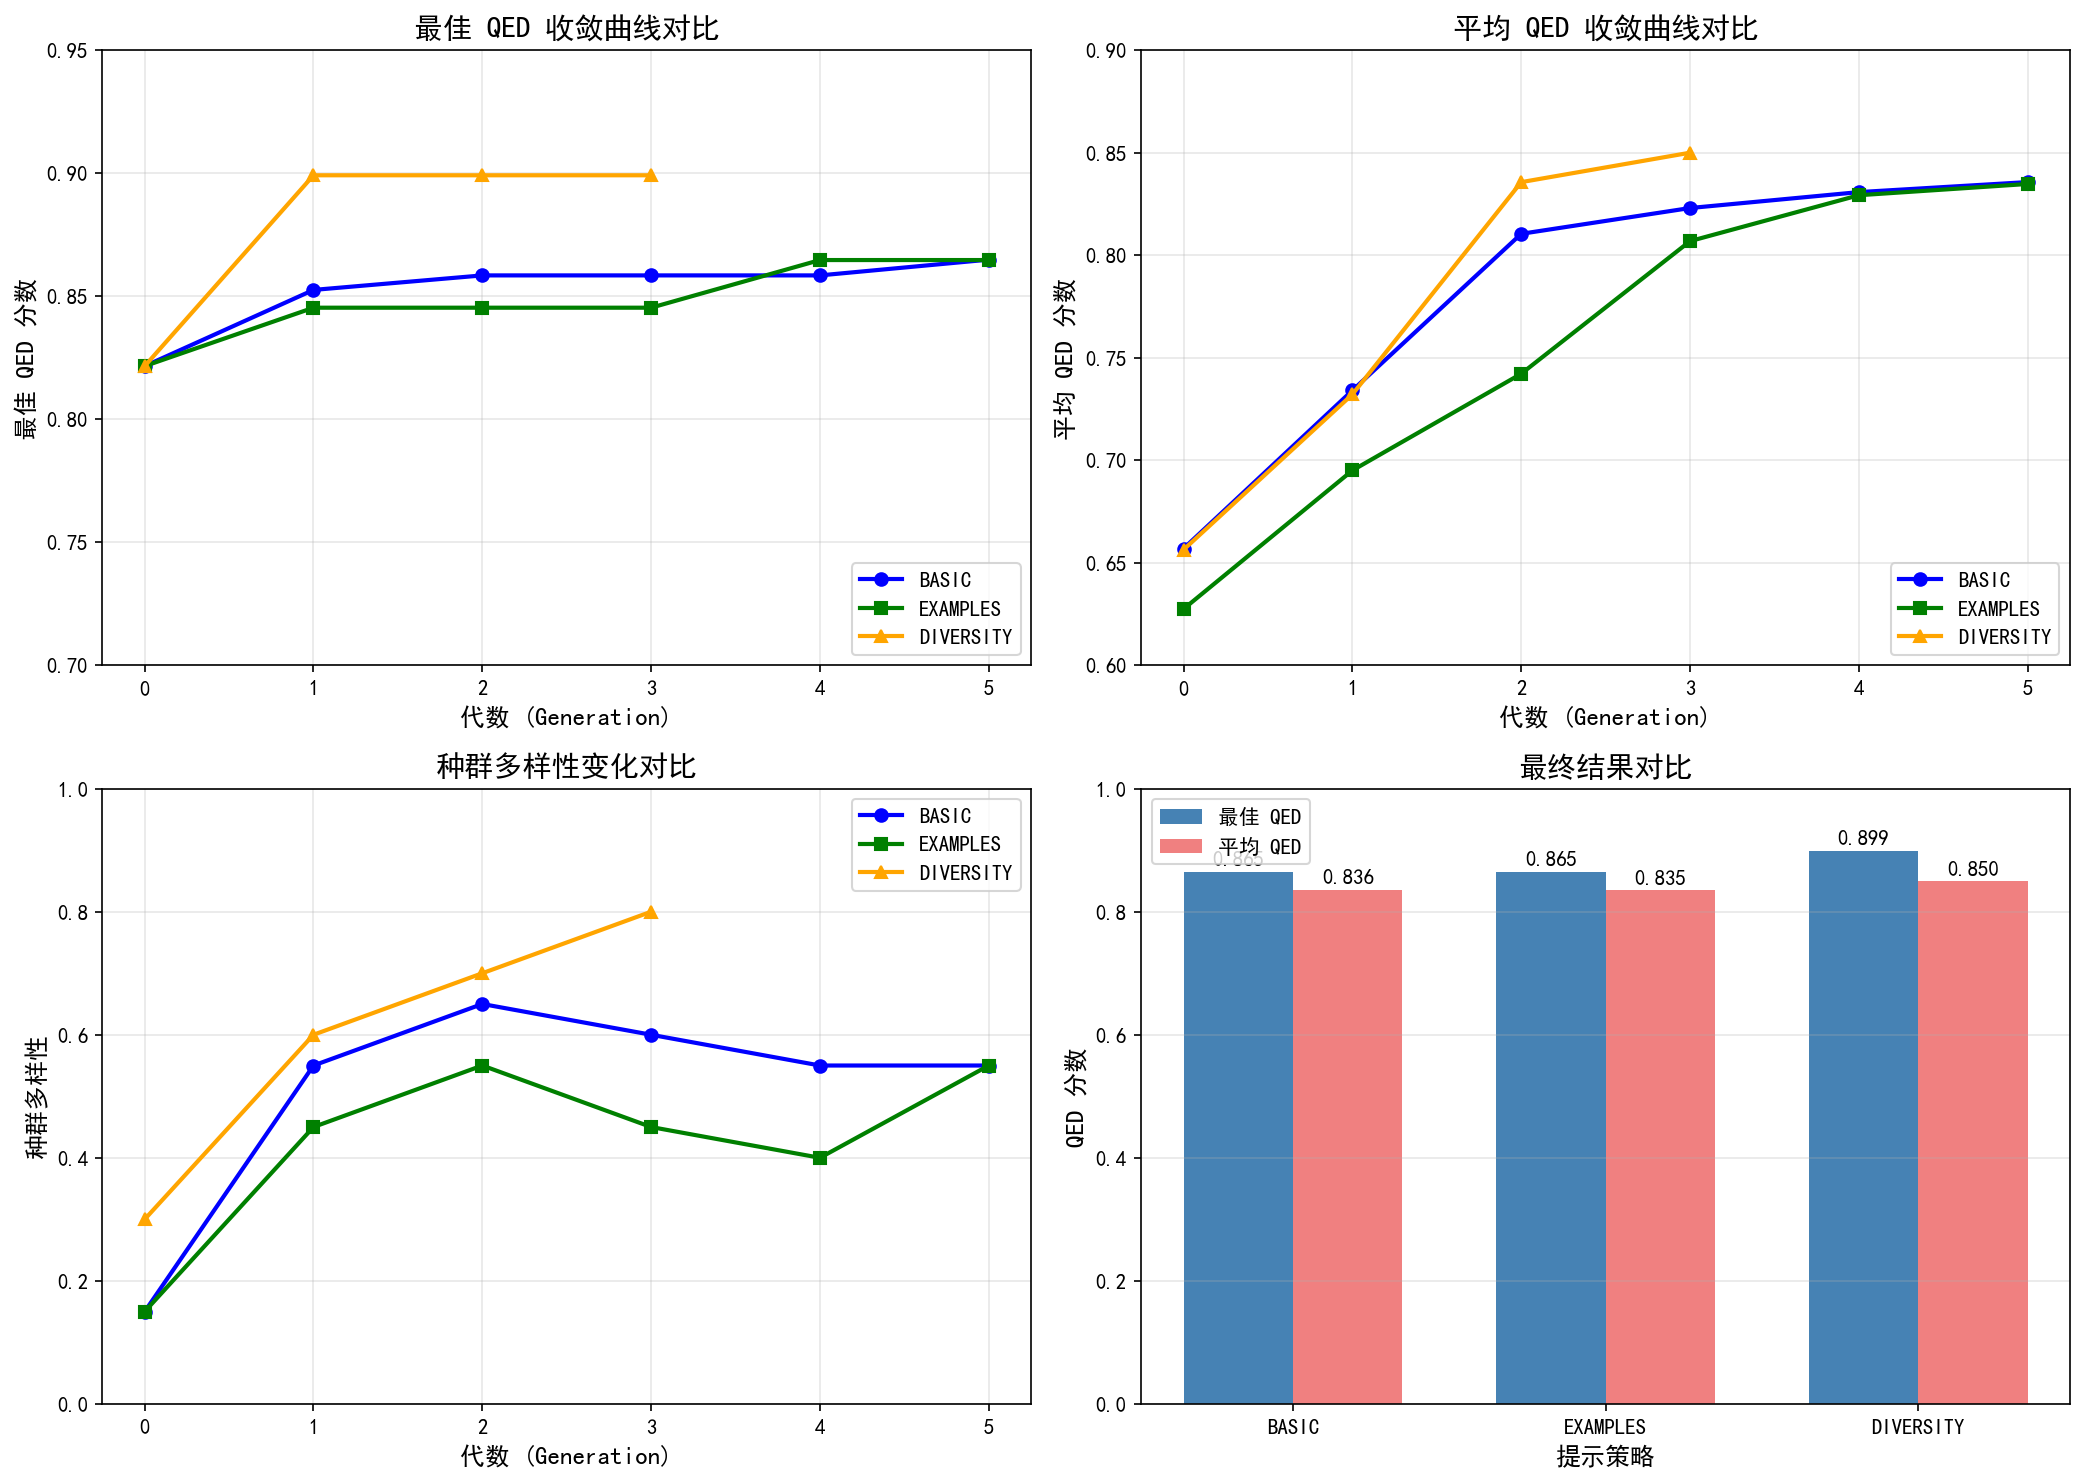
\includegraphics[width=0.95\linewidth]{convergence_comparison.png}
\caption{三种提示策略的对比实验结果}
\label{fig:convergence_comparison}
\end{figure}

\section{种群多样性分析}

种群的多样性是进化算法中的一个重要指标,它反映了搜索的广度和深度。如果多样性太高,说明种群过于分散,可能无法集中精力优化某个区域；如果多样性太低,说明种群过于集中,可能会陷入局部最优,无法找到更好的解。理想的状况是在前期保持较高的多样性,广泛探索搜索空间；在后期逐渐降低多样性,集中精力优化最有希望的区域。

在我们的实验中,我们通过计算每代的种群多样性(不同SMILES的比例)来监控多样性的变化。图4-2展示了三种策略的多样性随代数的变化曲线。从图中可以看到,所有策略在初期的多样性都很高,接近1.0,这是因为初始种群是随机采样的,几乎没有重复的分子。随着进化的进行,多样性逐渐下降,这是因为优秀的分子会被反复选择和复制,导致种群中出现越来越多的相似个体。

基础策略的多样性下降最快,在第10代时就降到了0.7左右,到第20代时降到了0.6以下。这说明基础策略很容易导致种群的聚集,所有的个体都朝着同一个方向进化,失去了探索其他区域的能力。这种现象在进化算法中被称为"早熟收敛"(Premature Convergence),是一个常见的问题。早熟收敛会导致算法陷入局部最优,无法找到全局最优解。

示例策略的多样性下降速度介于基础策略和多样性策略之间。在前10代,它的多样性保持得比较好,大约在0.8左右；但是从第15代开始,也开始快速下降,到第20代时降到了0.65左右。这可能是因为示例虽然提供了一些指导,但是并没有明确要求模型保持多样性,所以随着时间的推移,模型还是会倾向于生成相似的分子。

多样性策略的表现最好,它的多样性在整个进化过程中都保持在0.8以上,即使在第20代时,也有0.85左右。这说明多样性策略有效地抑制了种群的聚集,让模型持续地探索新的结构。多样性策略之所以能够做到这一点,是因为它在提示词中明确告诉了模型近期已经生成过的分子,并要求模型避免重复。这种"负反馈"机制让模型有意识地去尝试不同的结构,从而保持了多样性。

多样性的高低对优化效果有着直接的影响。我们从实验结果中看到,多样性策略不仅保持了更高的多样性,还取得了更好的QED分数。这说明在本研究的任务中,保持多样性是有利的,它能够帮助算法找到更好的解。当然,这并不是说多样性越高越好,如果多样性一直保持在1.0,说明种群完全没有收敛,可能也无法找到高质量的解。关键是要在探索(Exploration)和利用(Exploitation)之间找到平衡,这正是多样性策略所做的事情。

除了整体的多样性,我们还分析了分子结构的多样性。具体来说,我们使用RDKit的Scaffold功能来提取分子的骨架(Scaffold),然后统计不同骨架的数量。骨架是分子的核心结构,去掉侧链和官能团后剩下的部分。如果两个分子有相同的骨架,说明它们在结构上是相似的；如果有不同的骨架,说明它们属于不同的化学类别。我们发现,多样性策略生成的分子涵盖了更多的骨架类型,大约有15到20种不同的骨架；而基础策略和示例策略生成的分子主要集中在5到8种骨架上。这进一步证明了多样性策略在结构层面的有效性。

\section{随机性测试与稳定性分析}

大语言模型的生成过程本质上是随机的,即使是相同的输入,在不同的运行中也可能得到不同的输出。这种随机性来自于采样策略,特别是温度参数的设置。随机性既有积极的一面,也有消极的一面。积极的一面是它能够增加搜索的多样性,帮助算法跳出局部最优；消极的一面是它会导致结果的不确定性,使得实验难以复现,性能难以保证。

为了系统地研究随机性对优化过程的影响,我们设计了两个实验：一是温度参数的敏感性测试,二是多次独立运行的稳定性测试。

在温度参数的敏感性测试中,我们分别设置了四个不同的温度值：0.5、0.8、1.0、1.5,然后在相同的条件下运行优化算法,比较它们的结果。温度0.5代表较低的随机性,生成结果比较确定性；温度0.8是我们默认的中等随机性；温度1.0代表较高的随机性；温度1.5代表非常高的随机性,生成结果会很发散。实验的结果显示,温度对优化效果有着显著的影响。

当温度为0.5时,优化的过程非常稳定,每一代的最佳QED分数都在稳步提升,几乎没有波动。但是,最终的QED分数只有0.72左右,低于其他温度设置。这是因为低温度限制了模型的创造性,它只会生成与父代非常相似的分子,缺乏探索新结构的能力。种群的多样性也很低,只有0.5左右,说明种群很快就聚集在了一起。

当温度为0.8时,优化的过程也比较稳定,虽然有一些小的波动,但是总体趋势是向上的。最终的QED分数达到了0.80,是四个温度中最好的。多样性保持在0.8左右,说明既有一定的探索,又不至于太发散。这个结果验证了我们选择0.8作为默认温度的合理性。

当温度为1.0时,优化的过程开始出现较大的波动,有些代的最佳QED分数甚至会下降。最终的QED分数是0.78,略低于0.8的情况。多样性很高,达到了0.9左右,说明模型生成了很多不同的分子。但是,高多样性也意味着质量的参差不齐,有些分子很好,有些分子很差。

当温度为1.5时,优化的过程非常不稳定,最佳QED分数上下波动很大,没有明显的上升趋势。最终的QED分数只有0.70左右,是四个温度中最差的。多样性接近1.0,说明几乎所有的分子都是不同的,但是这些分子的质量普遍不高。这是因为过高的温度让模型的生成变得过于随机,失去了方向性,就像是在盲目地搜索,而不是有目的地优化。

从这四个温度的对比可以看出,温度参数的选择需要在稳定性和创造性之间做权衡。温度太低,稳定性好但是创造性不足；温度太高,创造性有余但是稳定性不够。0.8左右的温度是一个比较好的折中点,它既能保证一定的稳定性,又能提供足够的创造性。当然,这个最佳的温度值可能因任务和模型而异,在实际应用中,可以通过实验来确定最适合的温度。

在多次独立运行的稳定性测试中,我们使用相同的参数配置(温度0.8,多样性策略),进行了5次独立的运行,每次运行都使用不同的随机种子。我们记录了每次运行的最终最佳QED分数、平均QED分数、以及达到特定QED阈值(如0.75)所需的代数。结果显示,5次运行的最佳QED分数在0.78到0.82之间,平均值是0.80,标准差是0.015。这个标准差比较小,说明方法的稳定性是比较好的,不会因为随机性的影响而产生巨大的差异。

达到0.75 QED阈值所需的代数在12到18代之间,平均是15代。这也说明方法的收敛速度是比较稳定的,不会出现某次运行特别快或者特别慢的情况。从这些统计数据来看,我们提出的方法具有较好的可重复性和可靠性,这对于科学研究和实际应用都是非常重要的。

当然,我们也承认,大语言模型的随机性是一个需要持续关注和改进的问题。在未来的工作中,可以考虑引入更多的控制机制,比如自适应温度调整(根据优化的进展动态调整温度)、集成多个运行结果(取多次运行的最优解)、或者使用确定性更强的采样策略(如Beam Search)等,来进一步提高方法的稳定性和可控性。

\section{结果讨论}

综合以上的实验结果,我们可以得出以下几个重要的结论：

第一,大语言模型确实能够有效地用于分子优化任务。通过合适的提示词设计,大语言模型能够理解分子的结构和优化目标,并生成具有改进性质的新分子。这种方法的优势在于它不需要专门的训练,可以直接利用预训练模型的知识和能力,大大降低了应用的门槛。同时,自然语言的提示方式非常灵活,可以根据需要调整优化的目标和约束,比传统的固定算子更加通用。Yang等人\cite{yang2024llm}提出的OPRO方法也证明了LLM作为优化器的有效性,他们通过自然语言描述优化任务,让LLM自动寻找最优解。

第二,提示词的设计对优化效果有着至关重要的影响。我们的实验表明,不同的提示策略会产生截然不同的结果。基础的提示虽然能够完成任务,但是效果有限；加入示例可以提升前期的性能,但是后期的增益不明显；鼓励多样性的提示则能够全面提升优化的质量和稳定性。这说明,在使用大语言模型时,不能简单地把它当作一个黑箱,而是要精心地设计提示,充分发挥模型的能力。提示工程(Prompt Engineering)已经成为使用大语言模型的一项核心技能,值得深入研究和实践。Yoshikawa等人\cite{yoshikawa2025lico}提出的LICO方法也强调了上下文学习在分子优化中的重要性,通过在提示中加入相关示例,可以显著提升LLM的优化性能。

第三,保持种群多样性是成功的关键因素之一。在分子优化这样的复杂任务中,搜索空间非常大,而且充满了局部最优。如果过早地收敛到某个区域,很可能会错过更好的解。通过鼓励多样性,我们可以让算法持续地探索新的区域,增加找到全局最优的机会。我们的多样性策略通过在提示词中加入近期分子的信息,并要求模型避免重复,有效地实现了这一目标。这个思路可以推广到其他类似的优化问题中,具有重要的借鉴意义。

第四,大语言模型的随机性是一把双刃剑,需要合理地控制和利用。适度的随机性能够增加搜索的多样性,帮助跳出局部最优；但是过度的随机性会导致结果的不稳定,降低优化的效率。通过调整温度参数,我们可以在稳定性和创造性之间找到平衡点。在我们的实验中,0.8左右的温度表现最好,但是这个值可能需要根据具体的任务和模型进行调整。

第五,我们的方法虽然取得了一定的成果,但是还存在一些局限性和改进的空间。一是目前只优化了单一的QED属性,实际的药物设计需要考虑多个属性的平衡,如活性、选择性、毒性、合成可行性等。多目标优化是一个更具挑战性的问题,需要设计更复杂的提示策略和评价机制。二是大语言模型的生成效率还不够高,每次调用需要几秒钟的时间,对于大规模的优化任务来说,这可能成为瓶颈。未来可以考虑使用更快的模型、或者引入缓存机制来加速。三是分子的有效性还需要提高,目前有20\%-30\%的生成结果是无效的,这浪费了计算资源。可以通过改进提示词、或者使用后处理修正来提高有效率。四是缺乏与传统方法的直接对比,虽然我们引用了文献中的数据,但是最好能够实现一个传统的遗传算法作为基线,进行公平的比较。最近,Zhang等人的系统综述\cite{zhang2025survey}全面总结了LLM在进化优化中的应用,为未来的研究提供了重要的参考方向。Wang等人\cite{wang2025when}也详细分析了LLM与进化算法结合的潜在增强和挑战,指出了多个值得探索的研究方向。

尽管存在这些局限性,我们认为本研究的方向是有前景的。大语言模型在分子设计领域的应用才刚刚起步,还有很多值得探索的地方。随着模型能力的不断提升和方法的不断完善,我们相信这种基于自然语言的分子优化方法会在药物研发中发挥越来越重要的作用。
